\documentclass[12pt]{article}
\usepackage{import}
\usepackage{preamble}
\usepackage{environments}
%\usepackage{fourier}

%hspace before small will move the keywords around
\providecommand{\keywords}[1]
{
    \hspace*{0pt}\small	
  \textbf{\textit{Keywords--}} #1
}

\title{Geometric Algebra and Spinors}
\renewcommand{\maketitlehookb}{\centering Solving Problems in Applied Mathematics\\
Colorado State University}
\author{Colin Roberts}
\date{October 21$^\textrm{st}$ 2019}


\begin{document}

% Title Page
\begin{titlingpage}
    \maketitle
    \vfill
    \begin{abstract}
        The vector algebra of $\R^3$ given to us by Helmholtz is rather faulty.  We teach our students this language and we are able to perform computations, but is this really the right way? Clifford (not the Big Red Dog) would argue otherwise.  Rather, one can build a structure that contains not only the vector algebra in $\R^3$, but the exterior algebra in arbitrary dimension as well. Denote this new algebra as the geometric algebra $\nspacealg$. The goal of geometric algebra is to provide an algebraic (and smooth) structure that completely encodes the geometry of an underlying (quadratic) vector space but can extend to structures such as a Riemannian manifold. 
        
        In this talk, I will introduce the geometric algebras of 2-space $\twospacealg$ and of 3-space $\spacealg$.  We can see the usefulness in this perspective with examples from classical physics. For example, the central potential in the classical realm provoke the use of the real $\Spin(3,0)$ group to convert a nonlinear problem for a vector trajectory into a linear problem on a trajectory for a spinor. Hence, $\Spin(3,0)$ forms the bridge to the immensely important group $\Spin(p,q)$ seen throughout physics in the study of gravitation and quantum mechanics. 
    \end{abstract}
    %\vspace*{10pt}
    \keywords{geometric product, inner product, exterior product, grade, multivectors, pseudoscalar, rotor, spinor}
\end{titlingpage}


\section{Introduction}
\subsection{History}
There was quite a bit of history involved with the notion of vectors and vector calculus in the mid to late 1800's.  Different mathematicians had come up with unique ways of algebraically and analytically representing the geometry of space.  Most notably, we had Hamilton, Helmholtz, Grassmann, and Clifford.  Each had their own impact, but in some sense the notion of vector operations given by Helmholtz was what won out.  Around the same time, Hamilton had created the quaternions which, in some sense, better captured the geometry of space.  Grassmann had generated an exterior algebra of (what we now call) forms which was similar to both the vector and quaternionic view of Helmholtz and Hamilton respectively.  But, Clifford had actually created a structure that captured each one of these (as a substructure of something larger) and generalized it all beautifully. Here, we pay a slight homage to Clifford in his interpretation of the algebra of space.  

\subsection{Motivation}
In linear algebra and vector calculus we study products and derivatives of vectors and multivariate functions.  But, some of the operations we use in 3-space are unique to 3-space itself and hence do not generalize naturally.  We will find that this is mostly due to the fact that in 3-space, a vector uniquely defines a plane and vice-versa. Hence, we can be a bit sloppy with geometric products. We can gain much intuition from the geometry of the complex numbers and quaternions.  In fact, these are specifically examples of algebras of 1-space and 2-space respectively. Or, they can be seen as subalgebras of 2-space and 3-space respectively. This containment should be expected as well since there is, for example, a copy of 2-space living in 3-space.  

We must do away with the traditional vector interpretation in 3-space and instead consider a \emph{multivector} or \emph{geometric algebra} interpretation. This is not only a mathematical convenience for generalizing to higher dimensions, but it turns out to be computationally advantageous in, for example, computer vision.  Alongside that, it turns out to be a beautiful way to phrase physics such as classical mechanics, electromagnetism, or quantum mechanics.  In these realms of physics, we find structures such as \emph{spinors} or \emph{psuedoscalar} fields which are given a proper interpretation under geometric algebra. For example, spinors show up in classical mechanics as \emph{rotors} for central potential problems and these rotors appear again in the study of fermions.  The $\textrm{Spin}(n,0)$ Lie group (which double covers $\mathrm{SO}(n,0)$) can be thought of as the group of rotors on 3-space and, for example, the associated Lie algebra $\mathfrak{spin}(n,0)$ can be thought of as the algebra of \emph{bivectors}. Typically, one sees this Lie group defined differently and the associated Lie algebra defined with (somewhat unintuitive) Pauli matrices. 

Though we will not get into the full abstract construction of a \emph{Clifford algebra}, we do construct the geometric algebra of $n$-space, $\nspacealg$.  The notion of a Clifford algebra allows for one to create as a specific example the \emph{exterior algebra of differential forms} by use of a trivial quadratic form $Q$.  One could choose any quadratic vector space $(V,Q)$ and build a Clifford algebra.  A geometric algebra would then be formed by choosing a vector space $V$ and letting $Q$ be a (pseudo) inner product.  For example, one may wish to have an inner product $\langle \cdot, \cdot \rangle_g$ that varies from point to point in space as in a Riemannian manifold.  Similarly, one may be interested in the geometry of Minkowski spacetime where we only have a pseudo inner product with signature $(+,+,+,-)$.  

In this talk, we work towards an understanding of the calculus behind this vector algebra as well.  That is, we will investigate the rates of change of multivector fields and their interactions with other multivector fields.  Some worthwhile examples from classical mechanics and electromagnetism will (with enough time) be visited as well.  Many of us are familiar with Maxwell's equations in the vector (or Helmholtz) form and we will find that they can all be written as one multivector equation.  Not only is this compact, but it gives us a stronger understanding of the fields at hand. Special relativity tells us that electric fields and magnetic fields are unified together.  Geometric calculus in Minkowski space allows us to realize that the unification is simply a transformation of vector fields into bivector fields (boosts of electric fields produce magnetic fields).  

There are many reasons one should care about this subject.  I've only laid out a few that I have learned as of this time.  Let us venture into discovering more!

\emph{Note: If you attended my Greenslopes talk on the differential forms in $\R^3$, much of this will be familiar. If you'd like those notes as well, please email me.}

\subsection{Preliminaries}
% define algebras and relevant vector space stuff. Graded algebras. Examples with polynomials
put algebras as $\alg$ and define alg iso

\section{Geometric Algebra}
\subsection{Intuition from $\C$ and $\quat$}
For the majority of this talk, we consider the Euclidean inner product space $\R^3\equiv \left(\R^3,\cdot\right)$ which we will refer to as \boldblue{3-space}.  Similarly, we mean the Euclidean inner product space $\R^2\equiv \left( \R^2, \cdot\right)$ as \boldblue{2-space}. 

\begin{ex}{Complex Number Algebra}{complex_num_alg}
Let us begin with the motivating example of the complex numbers $\C$.  In this case, we write a complex number $z_1=x_1+iy_1$.  We can write another complex number as $z_2=x_2+iy_2$ and consider the product of these numbers
\[
z_1z_2 = (x_1+iy_1)(x_2+iy_2)= (x_1x_2 - y_1y_2)+i(y_1x_2+y_2x_1) = \RE(z_1z_2)+i\IM(z_1z_2).
\]
Notice that in this product, we end up with a complex number again and we can compute the entries for the resultant real and imaginary part.  We interject some notation that
\[
z_1z_2 = z_1\cdot z_2 + z_1 \wedge z_2
\]
where
\[
z_1 \cdot z_2 \coloneqq \RE(z_1z_2) \qquad \textrm{and} \qquad z_1 \wedge z_2 \coloneqq \IM(z_1z_2).
\]
Fundamentally, we notice that there is a splitting between real and imaginary parts for complex numbers in their multiplication.  One may also notice that the real part of the product $z_1\cdot z_2$ looks much like a dot product, but with an additional negative sign (due to $i^2=-1$). Similarly, $z_1\wedge z_2$ looks like the curl in 2-space but with an additional negative sign.
\end{ex}

\begin{ex}{Quaternion Algebra}{quat_alg}
The next motivating example is that of the \boldblue{quaternion algebra} $\quat$ given by
\[
\quat = \R \oplus \R i \oplus \R j \oplus \R k
\]
with the relations that
\[
i^2=j^2=k^2=ijk=-1.
\]
Consider two \boldblue{purely imaginary quaternions} $q,q'\in \quat$ with $q=ai+bj+ck$ and $q'=a'i+b'j+c'k$.  Then we can multiply these quaternions
\begin{align*}
    qq' &= (ai+bj+ck)(a'i+b'j+c'k)\\
    &= -(aa'+bb'+cc')+\left[(bc'-cb')i+(ca'-ac')j+(ab'-ba')k\right].
\end{align*}
This may look very familiar! Thinking of $q$ and $q'$ as vectors in 3-space (which they essentially are), we have
\[
qq' = -q\cdot q' + q\times q'.
\]
So, in some way, these quaternions capture both vector products we use in 3-space. To match notation from the previous example, one is inclined to replace $\times$ with $\wedge$.
\end{ex}

\subsection{Geometric Algebra of 2-Space}
Let us now build up the \boldblue{geometric algebra} of 2-space which we denote by $\twospacealg$.  We begin with an orthonormal basis of 2-space given by $e_1$ and $e_2$. We can generate a basis for $\twospacealg$ by considering some type of product between two vectors $\vectv,\vectw \in \twospacealg$. We can write each vector as a linear combination of the basis vectors by
\[
\vectv = v_1 e_1 + v_2 e_2 \qquad \textrm{and} \qquad \vectw = w_1 e_1 + w_2 e_2.
\]
We will end up treating the basis vectors in their own unique way as follows. So we define the \boldblue{geometric product} of $\vectv$ and $\vectw$ by
\begin{align*}
\vectv \vectw &\coloneqq (v_1e_1 + v_2 e_2)(w_1 e_1 + w_2 e_2)\\
&= (v_1e_1)(w_1e_1)+(v_1e_1w_2e_2)+(v_2e_2)(w_1e_1)+(v_2e_2)(w_2e_2)\\
&= v_1w_1 e_1^2 + v_2w_2 e_2^2 + v_1w_2 e_1 e_2 + v_2w_1 e_2 e_1\\
&= (v_1w_1+v_2w_2)1 + (v_1 w_2 - v_2w_1)e_1\wedge e_2.
\end{align*}
We reduced this far by defining
\[
e_i^2 = e_i\cdot e_i = 1 \qquad \textrm{and} \qquad e_1e_2 = e_1\wedge e_2 = -e_2\wedge e_1=-e_2 e_1.
\]
Above, we let $\wedge$ denote the \boldblue{exterior product} of two vectors and $\cdot$ is the usual Euclidean \boldblue{inner product}. Maybe now these names seem to be a bit more related! Also, it should be noted that we can replace $e_1\wedge e_2$ by $e_1e_2$ itself since we chose our basis to be orthonormal. We will stick with orthonormal bases for the sake of ease (and since it is always possible to chose an orthonormal basis for an inner product space).

\begin{remark}{}{remark_basis}
As a side note, if we chose an arbitrary basis $b_1, b_2$ for 2-space, then we define
\[
b_1b_2 = b_1\cdot b_2 + b_1\wedge b_2.
\]
Hence, if $b_1$ and $b_2$ are orthonormal, $b_1\cdot b_2=0$ and we recover what we have above.
\end{remark}

So now, in $\twospacealg$ we have generated new basis elements $1$ and $e_1\wedge e_2$ for the vector space $\twospacealg$. We refer to $1$ as the \boldblue{scalar} and $e_1\wedge e_2$ as the \boldblue{bivector}. If we extend this geometric product to these new elements, we find that there are no new (vector) basis elements to generate. \emph{Note: the algebra basis of $\twospacealg$ is $\{e_1,e_2\}$ whereas the vector basis is $\{1,e_1,e_2,e_1\wedge e_2\}$.} 

\begin{ques}{How can we extend the geometric product?}{extend_geo_prod}
Say we want to define the geometric product on not just vectors, but on the scalar element $1$ and bivector element $e_1\wedge e_2$, how can we do this?
\tcblower
\begin{answer*}
We simply define the multiplication for all basis elements.  That is
\begin{align*}
    1 e_i &= e_i 1 = e_i\\
    e_1 (e_1 \wedge e_2)&=e_1e_1e_2 = e_1^2 e_2 = e_2\\
    e_2 (e_1 \wedge e_2)&= -e_2 (e_2\wedge e_1)=-e_2e_2 e_1 = -e_2^2e_1=-e_1\\
    (e_1\wedge e_2)(e_1\wedge e_2)&= -(e_1\wedge e_2)(e_2\wedge e_1)=-e_1e_2e_2e_1=-e_1e_1=-1.
\end{align*}
\end{answer*}
\end{ques}



\begin{prop}{$\twospacealg$ Contains the $\C$-Algebra}{twospacealg_iso_quat}
    The 2-space algebra $\twospacealg$ contains a copy of $\C$ as the subalgebra generated by $\{1, e_1\wedge e_2\}$. In other words, the \emph{\boldblue{even subalgebra}} of $\twospacealg$ is isomorphic to $\C$.
    \tcblower
    \begin{proof}
    Denote $I\coloneqq e_1\wedge e_2$ and consider two elements $z_1=1x_1+Iy_1$ and $z_2=1x_2+Iy_2$ in the subalgebra. Then
    \[
    z_1 z_2 = 1(x_1x_2 - y_1y_2)+I(y_1x_2+y_2x_1).
    \]
    This is the exact multiplication as $\C$ if we map $1\to 1$ and $I \to i$.  
    \end{proof}
\end{prop}

\begin{remark}{}{Quaternion_iso}
It turns out that the algebra of 2-space $\twospacealg$ is almost algebra isomorphic to $\quat$ itself.  In some sense, $\quat$ is a ``left-handed" algebra where as $\twospacealg$ is ``right-handed." One can also think of $\quat$ as the algebra with a psuedo inner product with signature $(-,-)$ instead of the typical inner product with signature $(+,+)$.
\end{remark}

Again, the vector basis for $\twospacealg$ is $\{1,e_1,e_2,e_1\wedge e_2\}$. Note that there is $1 = \binom{2}{0}$ scalar, $2=\binom{2}{1}$ vectors, and $1=\binom{2}{0}$ bivectors. When working in higher dimensional spaces, we need a term to refer to objects built from products of vectors.  The term we use is \boldblue{grade} which refers to the number of independent vectors present in an element of the geometric algebra.  For example, the scalar 1 is grade-0, the vectors are grade-1, the bivector is grade-2. We can also refer to $I=e_1\wedge e_2$ as the \boldblue{pseudoscalar} as it is the highest grade element in $\twospacealg$.

\subsection{Geometric Algebra of 3-Space}
3-space is spanned by the orthonormal basis vectors $e_1$, $e_2$, and $e_3$.  We wish to generate the geometric algebra of 3-space $\spacealg$ in the same way we generated $\twospacealg$.  So we can consider products of the basis vectors
\[
e_i^2 = 1 \qquad \textrm{and} \qquad e_ie_j = e_i\wedge e_j = -e_j\wedge e_i = -e_je_i ~\textrm{for $i\neq j$}.
\]
This gives us the scalars, vectors, and bivectors respectively
\[
1,e_1,e_2,e_3,e_1\wedge e_2, e_1\wedge e_3,e_2\wedge e_3.
\]
From vectors and bivectors we can generate a single trivector
\[
e_1\wedge e_2 \wedge e_3.
\]
Then we have a vector basis for the whole 3-space algebra $\spacealg$ given by
\begin{itemize}
    \item One Scalar: 1.
    \item Three Vectors: $e_1$, $e_2$, $e_3$.
    \item Three Bivectors: $e_1\wedge e_2$, $e_1 \wedge e_3$, $e_2\wedge e_3$.
    \item One Trivector (Psuedoscalar): $I=e_1\wedge e_2 \wedge e_3$.
\end{itemize}
Notice that the amount of grade-$k$ elements is given by the binomonial coefficient $\binom{n}{k}$ where $n$ is the dimension of the relevant space (in this case $n=3$). One may also notice that the vector space dimension of the geometric algebra of $n$-space $\dim_V\left( \nspacealg\right) = 2^n$ (which gives us $2^3=8$ for our case).

It's worth working through a few examples and performing the multiplication in $\spacealg$.  In this algebra, the most general element is a \boldblue{multivector} will come as the form
\[
M = \alpha + a + B + \beta I
\]
where $\alpha$ is a scalar, $a$ a vector, $B$ a bivector, and $I$ is the pseudoscalar. Given this, we also introduce the notation
\[
\langle M \langle_k 
\]
which outputs the grade-$k$ part of a multivector. For example, we have
\[
\langle M \rangle_0 = \alpha \qquad \langle M \rangle_1 = a \qquad \langle M \rangle_2 = B \qquad \langle M \rangle_3 = \beta I.   
\]
It suffices to multiply single objects of possibly different grade as this will extend to the multiplication properties for general multivectors. Prior to this, let us quickly reintroduce the inner product $a\cdot b$ and the outer product $a\wedge b$.  The inner product is a familiar Euclidean concept, and the outer product is defined above, but in general it simply satisfies the rule
\[
a\wedge b = -b\wedge a
\]
which further implies the rule
\[
a\wedge a = 0.
\]
Note that both the inner and outer product are linear in that
\[
a\cdot(b+ c) = a\cdot c + b \cdot c \qquad \textrm{and} \qquad a\wedge(b+c) = a \wedge c + b \wedge c.
\]
We can extend the notion of the inner and outer product to higher grade elements. How may we do so in a natural way? We can note that
\[
a\cdot b = \frac{1}{2}(ab + ba) \qquad \textrm{and} \qquad a\wedge b = \frac{1}{2}(ab-ba),
\]
which defines the inner and outer product for any two elements of the geometric algebra.

\begin{ex}{Multiplication of Elements of the Same Grade}{mult_of_grade_elements}
    \begin{itemize}
        \item \textbf{Scalars:} Multiplying scalars is familiar. If we take two scalars $\alpha$ and $\beta$ then $\alpha \beta$ is also a scalar. In fact, if we take a scalar times an element of any grade, it scales that element as expected. 
        \item \textbf{Vectors:} Let $a$ and $b$ both be vectors, then if we write these in terms of the standard basis 
        \begin{align*}
            a &= a_1 e_1 + a_2 e_2 + a_3 e_3 \\
            b &= b_1 e_1 + b_2 e_2 + b_3 e_3,
        \end{align*}
        we can use our multiplication rules to find
        \[
        ab = a\cdot b + a\wedge b. \footnote{Using the orthonormal basis above, one can realize the inner and outer product in terms of that basis. The inner product is a familiar computation, and the outer product can be computed using the above rules and verified by any source that mentions the exterior algebra.}
        \]
        Thus, the geometric product $ab$ splits into the inner and outer product. We also can note that the product of two grade-1 elements products a grade-0 element $a\cdot b$ and a grade-2 element $a\wedge b$.  In other words,
        \[
        \langle ab \rangle_0 = a\cdot b \qquad \textrm{and} \qquad \langle ab \rangle_2 = a\wedge b.
        \]
        \item \textbf{Bivectors:} Let us work with the basis bivectors
        \[
        B_1 = e_2 \wedge e_3 \qquad B_2 = e_3 \wedge e_1 \qquad B_3 = e_1 \wedge e_2,
        \]
        then it suffices to work out the multiplication of the basis bivectors since all bivectors are a linear combination of these basis elements. We in fact have
        \[
        B_i B_j = -\delta_{ij} -\varepsilon_{ijk}B_k,
        \]
        where $\delta_{ij}$ is the \boldblue{Kronecker delta symbol} that satisfies 
        \[
        \delta_{ij} = \begin{cases} 1 & \textrm{if $i=j$}\\ 
        0 & \textrm{if $i\neq j$} \end{cases}
        \]
        and $\varepsilon_{ijk}$ is the \boldblue{Levi-Civita symbol} that satsifies
        \[
        \epsilon_{ijk} = \begin{cases} +1 & \textrm{if $ijk$ is an even permutation of $123$}\\ 
        -1 & \textrm{if $ijk$ is an odd permutation of $123$}\\
        0 & \textrm{otherwise}\end{cases}.
        \]
        \item \textbf{Pseudoscalar:} We have the single pseudoscalar (the trivector in $\spacealg$) element $I=e_1\wedge e_2 \wedge e_3$. The pseudoscalr can then by squared to find that
        \[
        I^2 = II = (e_1 \wedge e_2 \wedge e_3)(e_1 \wedge e_2 \wedge e_3) = -1.
        \]
        This is true for the pseudoscalar in all dimensions. Note that we saw this quality in 2-space as well.
    \end{itemize}
\end{ex}
\newpage

Next, one could investigate products of different grade elements. That is, one could consider products of vectors with bivectors, vectors with the psuedoscalar, or bivectors with the pseudoscalar.  Instead of halting to compute these products now, we'll deal with these if they arise.

\subsection{Interpretation of Quantities}
After developing this algebraic structure, one may ask for a means for interpreting the different quantities.  This is of course a very natural question to ask.  We choose to impose a both a geometrical and physical interpretation to the different grade elements. Sticking with 3-space for now, we can assign the following meanings:
\begin{itemize}
    \item Grade-0: Scalar elements.
    \item Grade-1: Oriented length elements (directed line segments).
    \item Grade-2: Oriented area elements (oriented parallelograms).
    \item Grade-3: Oriented volume elements (oriented parallelepipeds).  
\end{itemize}
We are all familiar with scalar elements, and oriented length elements (which we typically think of as vectors anyway).  So, we really just need to more accurately describe the grade-2 and grade-3 objects.  Let us consider abstractly two vectors $a$ and $b$. Then we can form their exterior product $a\wedge b$ which is a grade-2 element.  We can picture this as follows:
\begin{figure}[H]
    \centering
    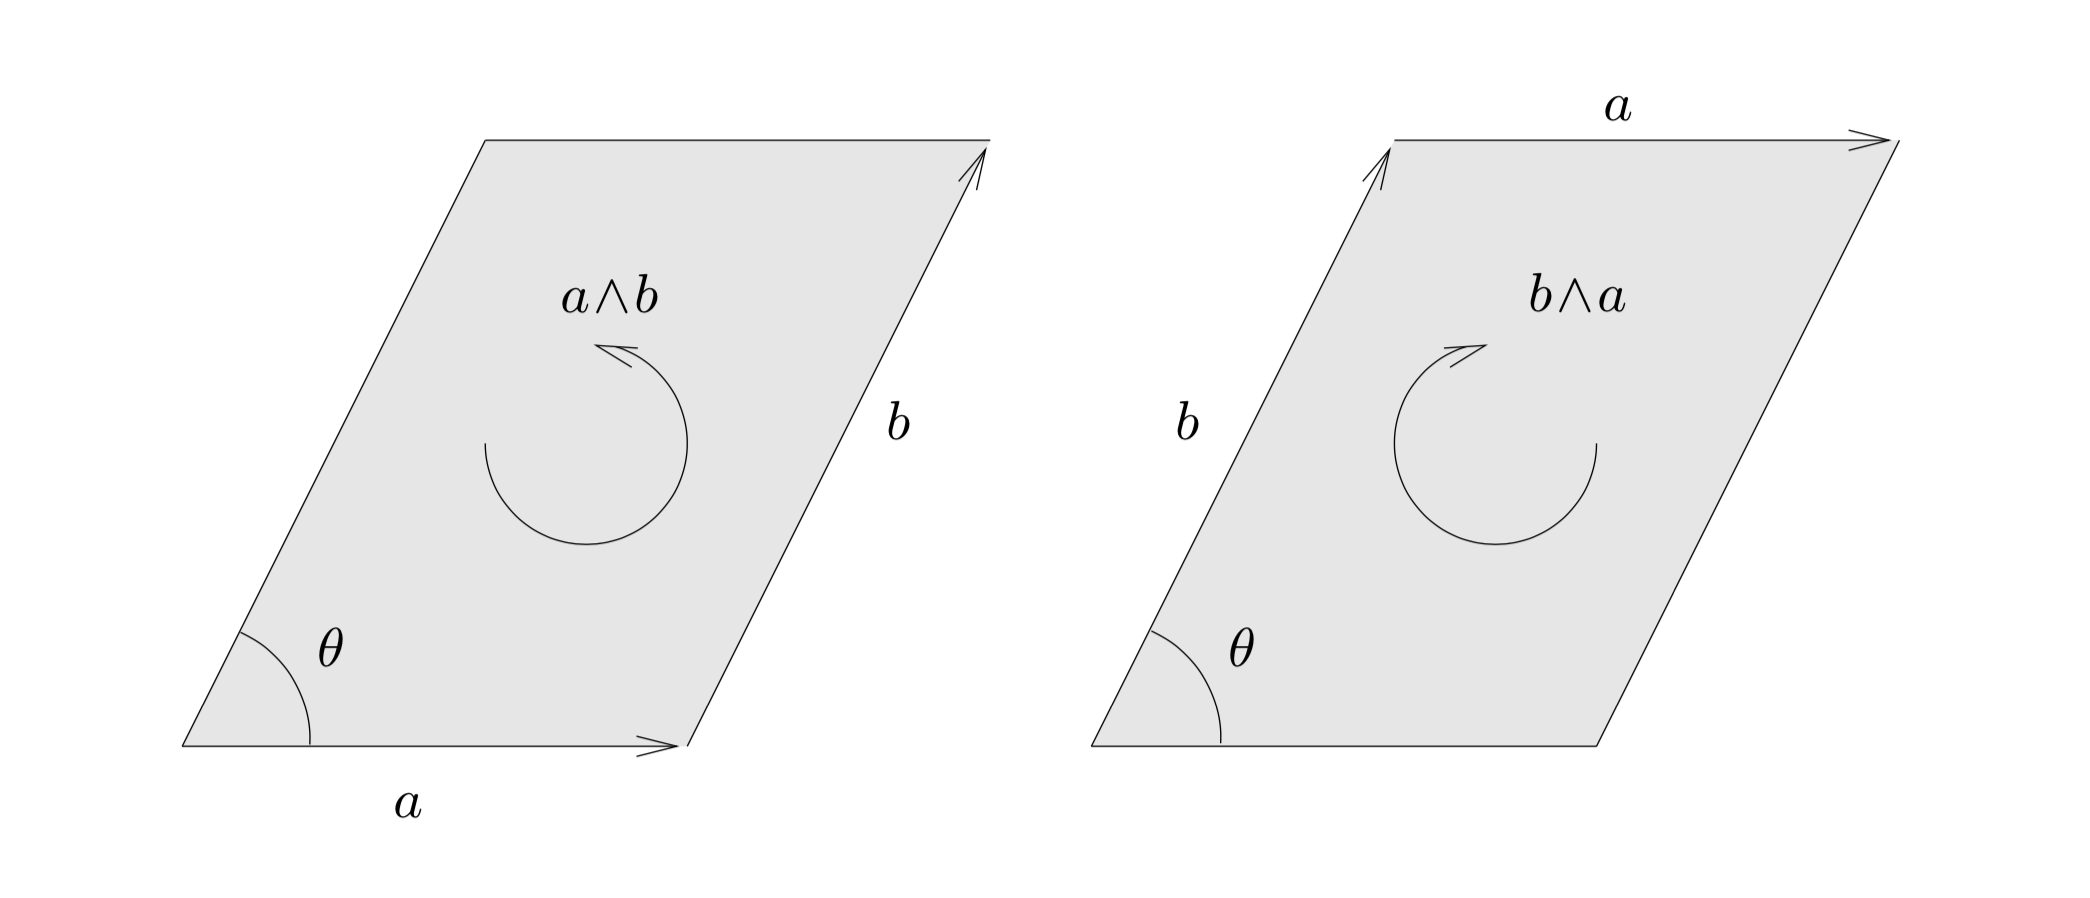
\includegraphics[width=\textwidth]{geometric_algebra_calculus/figures/ab_outer_prod.png}
    \caption{The outer product of vectors $a$ and $b$. Note the orientation induced by the order of the products.}
    \label{fig:bivector}
\end{figure}
The linearity of the outer product relates the addition of bivectors quite nicely.  That is, when we have
\[
a \wedge (b+c) = a\wedge b + a \wedge b
\]
we can realize this picture geometrically as follows:
\begin{figure}[H]
    \centering
    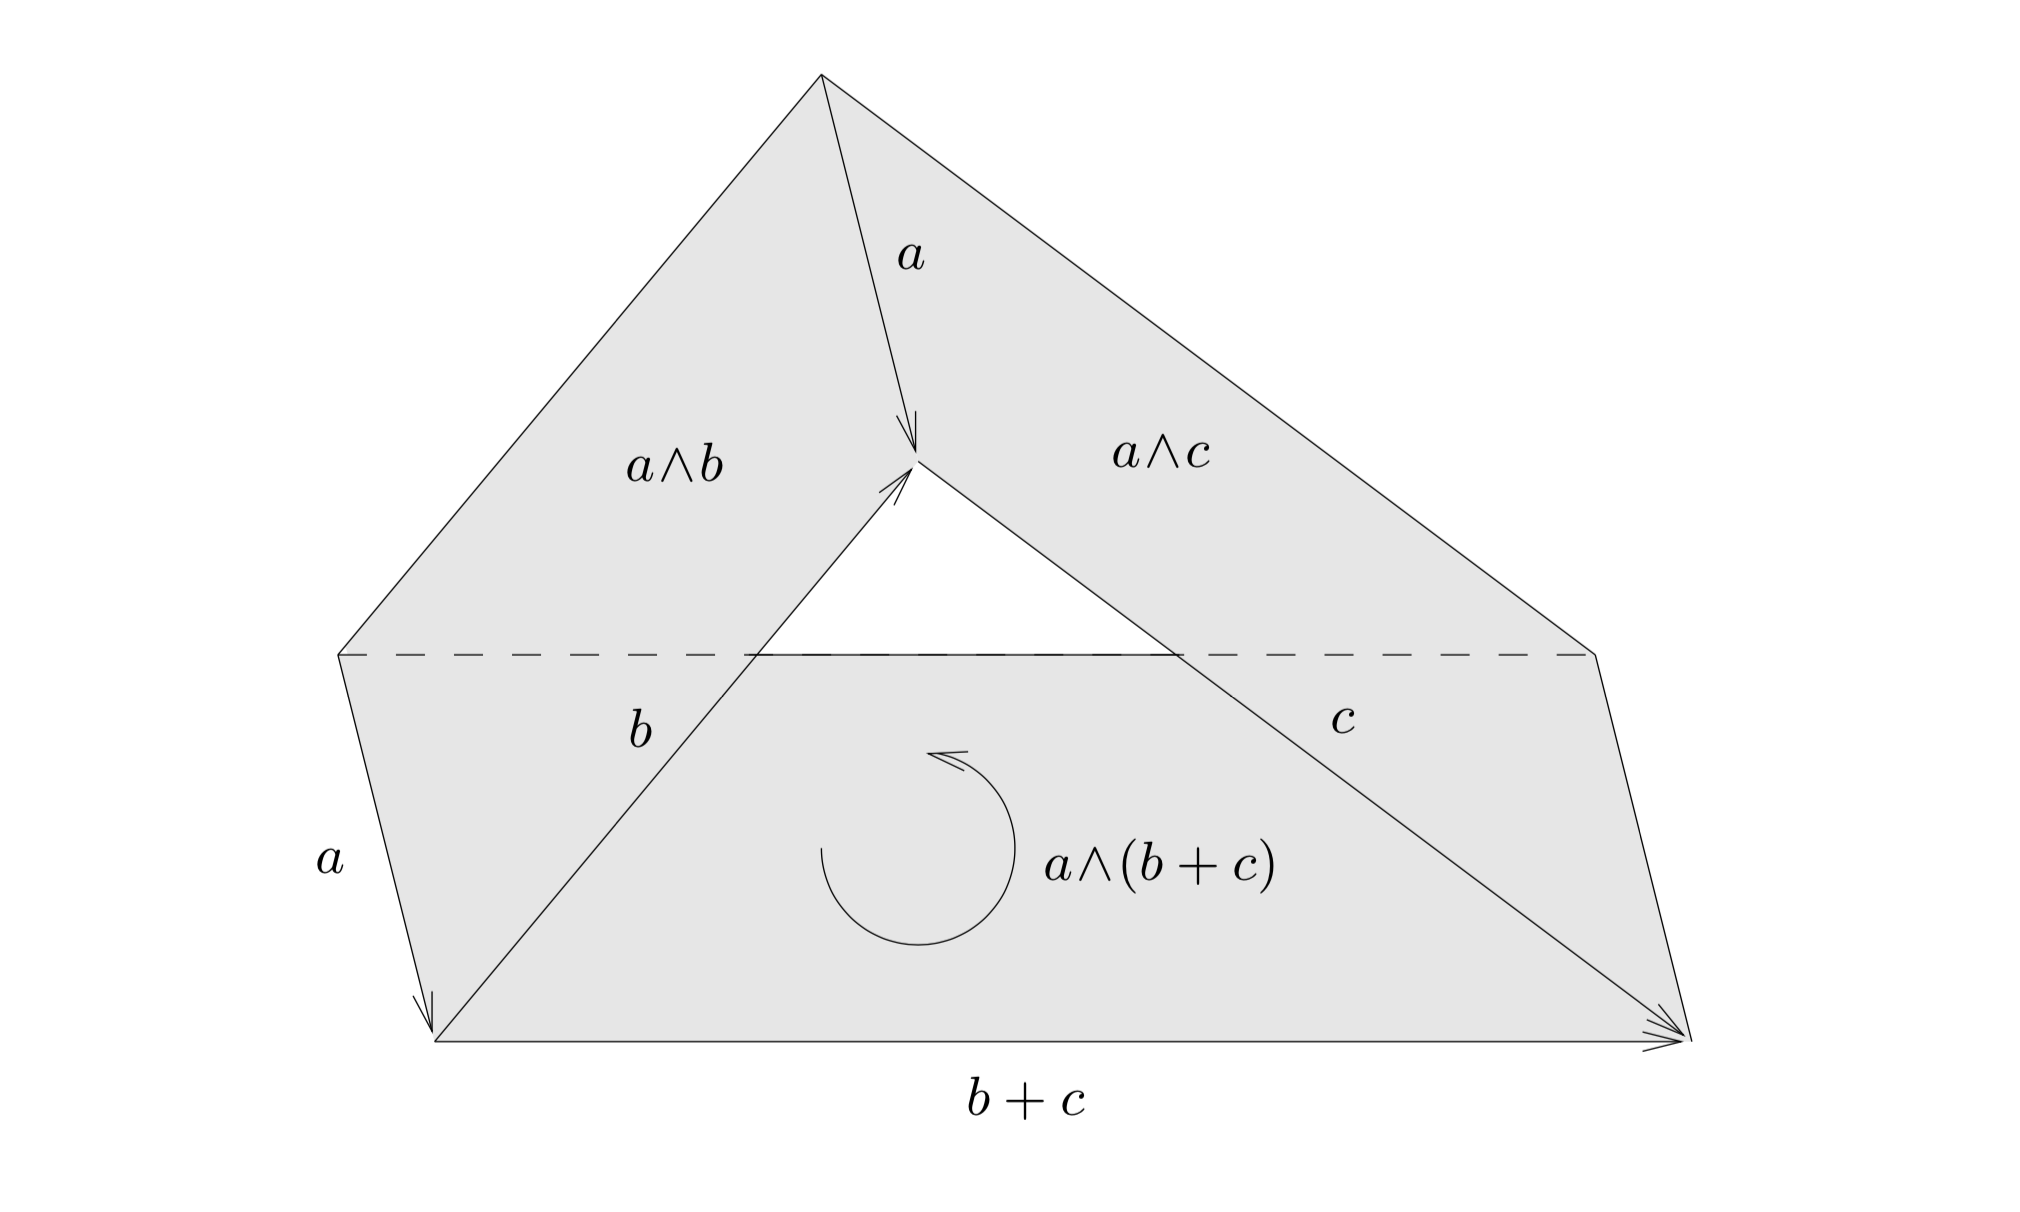
\includegraphics[width=\textwidth]{geometric_algebra_calculus/figures/linearity_out_prod.png}
    \caption{}
    \label{fig:bivector_linearity}
\end{figure}
We can then deduce the structure of a trivector in 3-space $a\wedge b \wedge c$ by the following figure:
\begin{figure}[H]
    \centering
    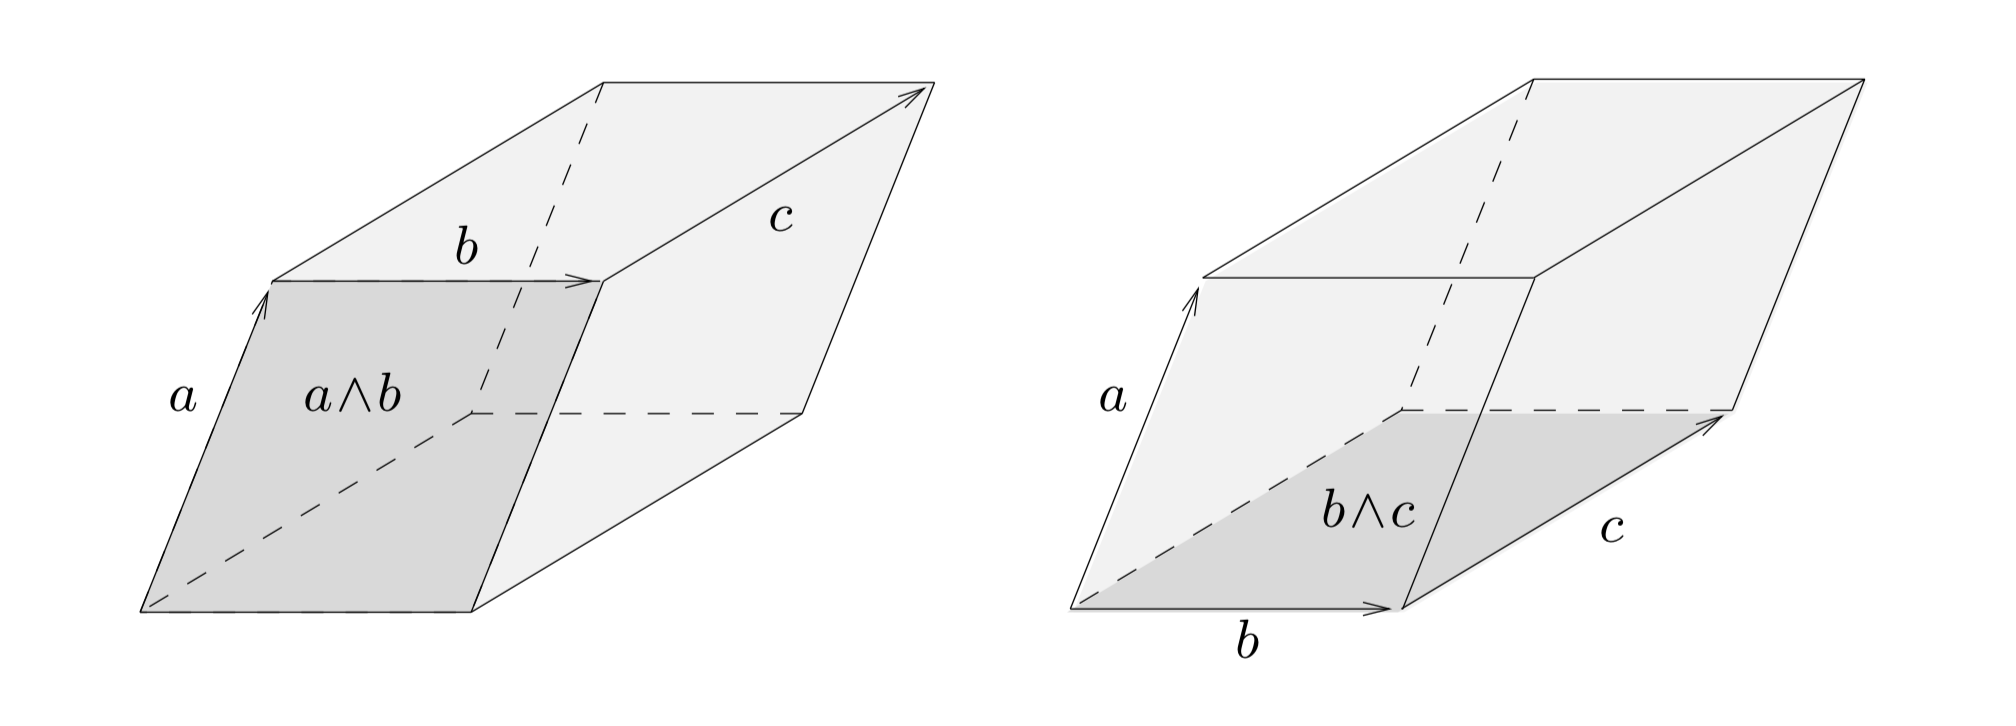
\includegraphics[width=\textwidth]{geometric_algebra_calculus/figures/trivector.png}
    \caption{The trivector $a\wedge b \wedge c$ given by the outer product of the three vectors $a$, $b$, and $c$.}
    \label{fig:trivector}
\end{figure}


%\subsection{Multivectors}

\subsection{Reflections and Rotations}

The major claim is that the geometric algebra captures ``all" the geometry of the underlying space.  If that's the case, one should definitely expect the algebra to capture actions like reflections and rotations. As it turns out, these are performed quite easily. We will stick with the case of 3-space, but this all generalizes to $n$-space of arbitrary (non-degenerate) signature.  Also, we will perform these actions on vectors for the sake of visualization as well, but each can be performed on elements of arbitrary grade.

Let $m$ and $a$ be a vectors in $\spacealg$ with $m^2 = 1$ so that $m$ is a unit vector.  Then we can define a \boldblue{reflection} of $a$ in the plane perpendicular to $m$ by
\[
b=-mam,
\]
where we put $b$ as the reflected vector. In higher dimensions, reflections are performed over hyperplanes which a vector $m$ can uniquely define. 

\boldblue{Reflections} are simply products of two reflections.  Hence, we choose another vector $n$ that also satisfies $n^2=1$, we can create a \boldblue{rotor} $R=nm$ that rotates a vector $a$ by the action
\[
c = RaR^\dagger = (nm)a(mn),
\]
where $\dagger$ reverses the order of vectors present in $R$. That is, we have
\[
(n_1 \dots n_k)^\dagger = n_k \dots n_1.
\]
This creation of a rotor allows us to understand rotations in arbitrary dimensions with a nice geometrical picture.  First, if we have $R=nm$, then
\[
R = nm = n\cdot m + n\wedge m,
\]
and we note that $n\wedge m$ defines the plane in which we rotate a vector $a$.  Then, the quantity
\[
n\cdot m = \cos \frac{\theta}{2},
\]
defines the angle in which we rotate the vector $a$ in the given orientation provided by $m\wedge n$.  Note that since we perform a two sided operation, we end up rotating by an angle of $\theta$ although $\theta/2$ appears throughout. Now, we have no need for an axis of rotation! However do note the slight reversion on the wedge. This gives us the decomposition
\[
R=\cos \frac{\theta}{2} - B \sin \frac{\theta}{2}
\]
where
\[
B=\frac{m\wedge n}{\sin \frac{\theta}{2}}.
\]
We can picture the rotation as follows:
\begin{figure}[H]
    \centering
    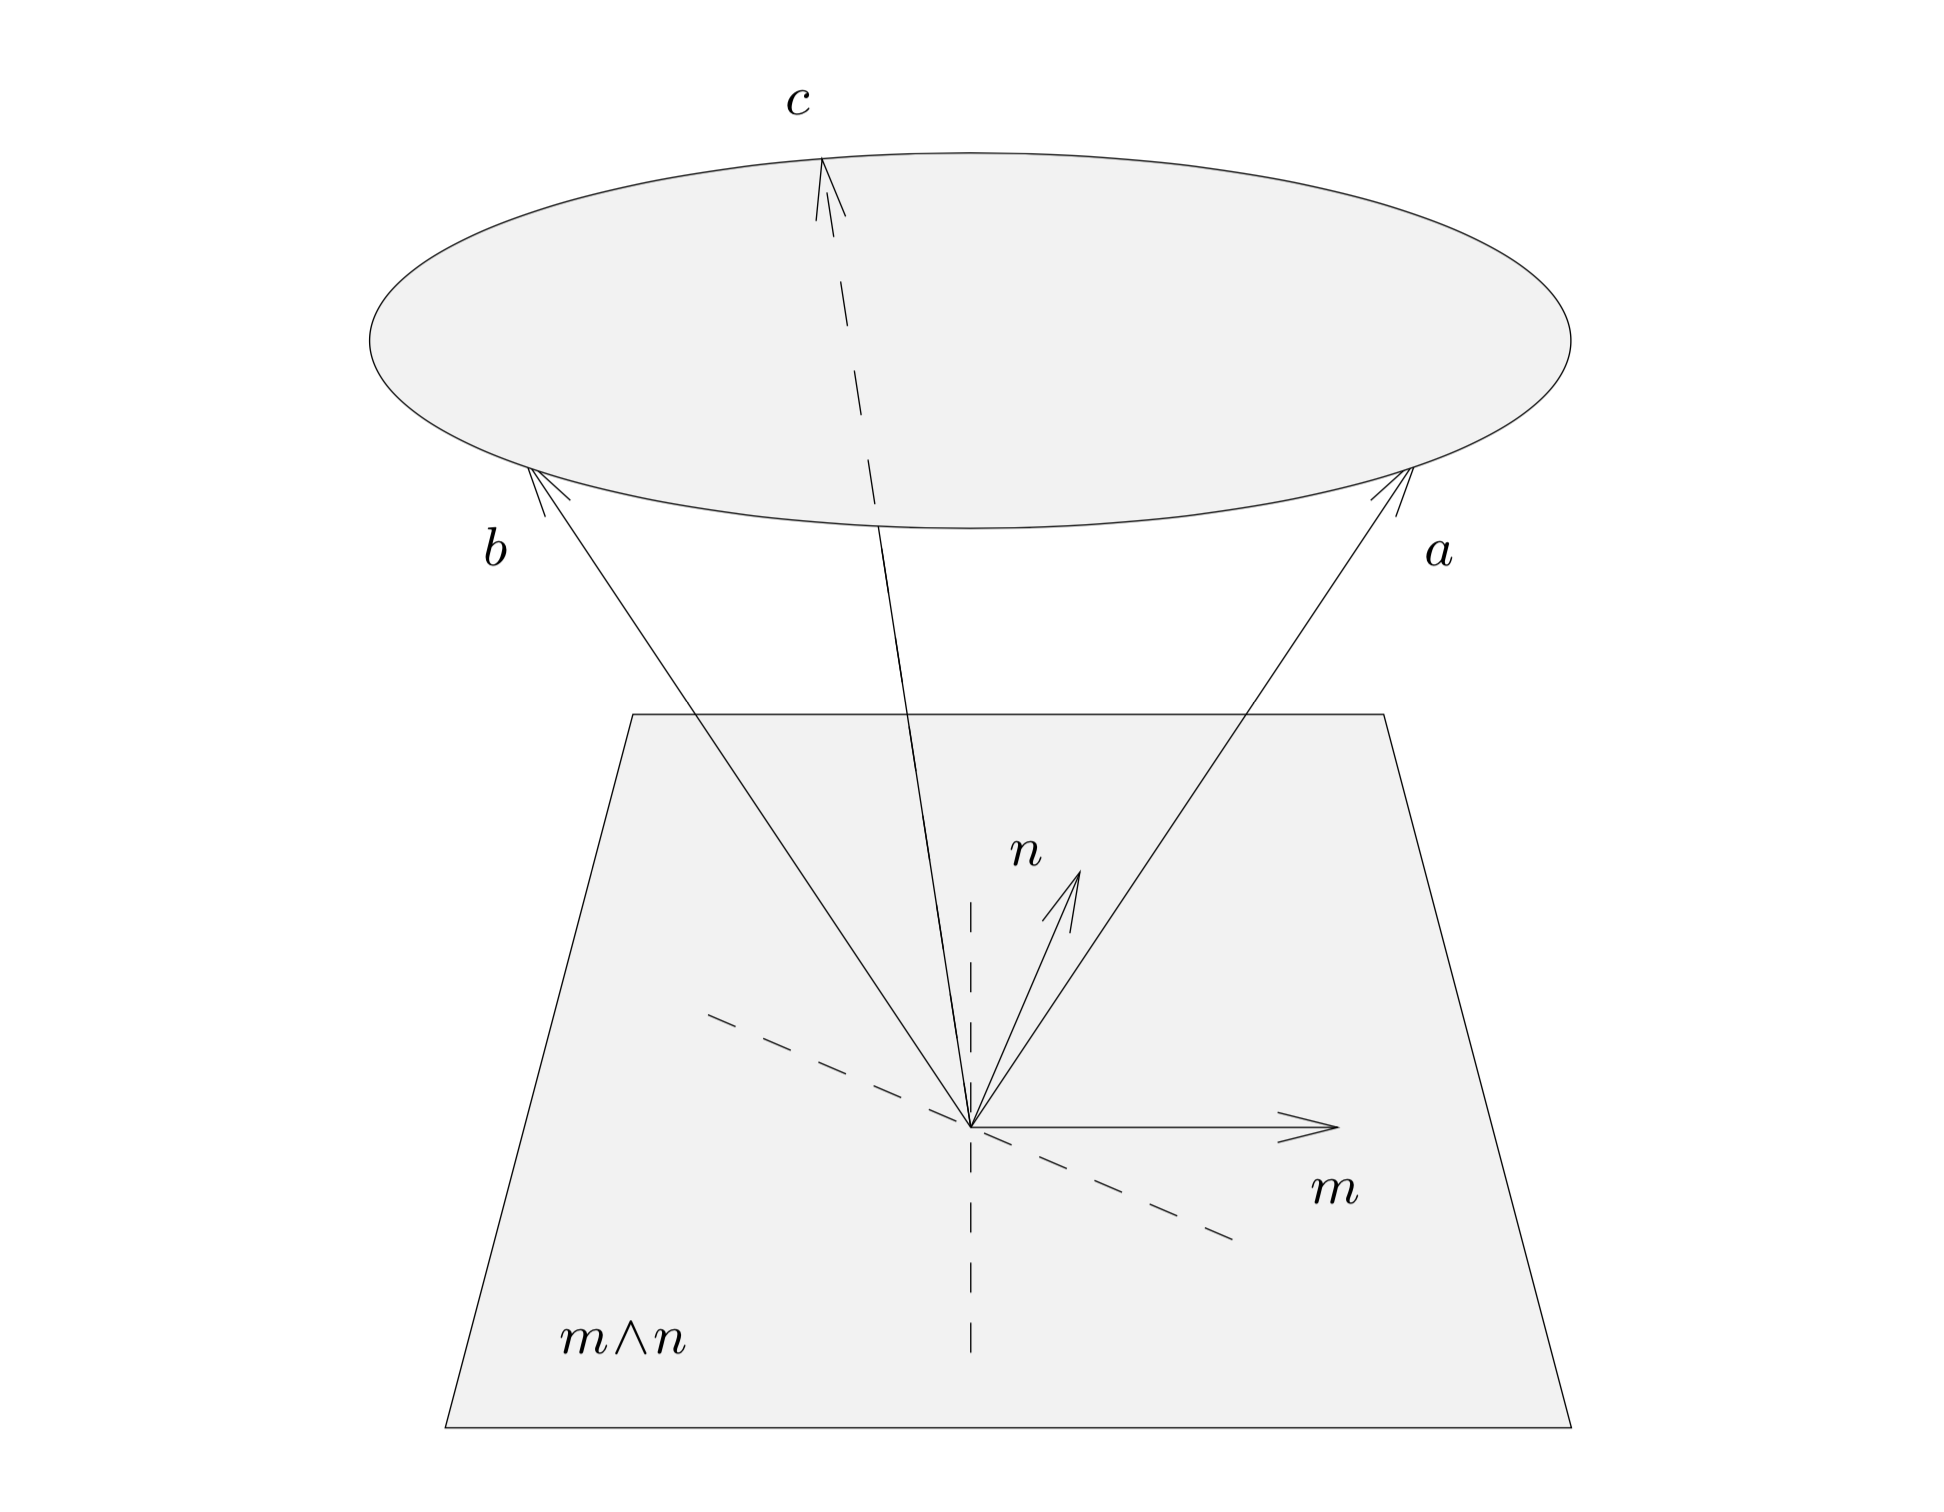
\includegraphics[width=.8\textwidth]{geometric_algebra_calculus/figures/rotation.png}
    \caption{A rotation of the vector $a$ to the vector $c$. Note that $b$ is the reflection of $a$ over the hyperplane defined by $m$ shown previously.}
    \label{fig:rotors}
\end{figure}

For the next wonderful property, we seek to remind ourselves of unit complex numbers.  Remember, we can write unit complex numbers as
\[
e^{i\theta}
\]
where $\theta$ describes the angle of rotation.  Recall that we can think of $i\equiv e_1 \wedge e_2$ as a part of the even subalgebra in $\twospacealg$ and we find
\[
R = \exp (-B\theta/2) = 1 + -B\theta + \frac{(-B\theta/2)^2}{2!}+\cdots.
\]
Hence, rotors are exponentials of bivectors!

Lastly, we remark that rotors form a group under composition. That is, given two rotors $R_1$ and $R_2$, we can create a product rotor $R$ by
\[
R = R_2\circ R_1
\]
where we define the action of $R$ on $a$ by
\[
a \mapsto RaR^\dagger = (R_2 R_1)a(R_2 R_1)^\dagger = R_2 R_1 a R_1^\dagger R_2^\dagger.
\]
This group of rotors turns out to be a fairly important group in a mathematical and physical way.  Specifically, this group of rotors we just discovered inside of $\spacealg$ is $\Spin(3)$.

\subsection{Spinors}

When reading of \boldblue{spinors}, they find that they are elements of spin groups. Then, one is pointed to the real $\Spin(n)$ group or, more generally, the $\Spin_\mathbb{F}(p,q)$ group over a field $\mathbb{F}$ with signature $(p,q)$. In the general case, we denote the \boldblue{signature} of an (pseudo)inner product to be $(p,q)$ if we have
\[
a\cdot b = \sum_{j=1}^p a_ib_i - \sum_{k=p+1}^{p+q}a_kb_k.
\]
The typical example for a space with a $p,q$ signature is that of \boldblue{Minkowski spacetime}.  We let Minkowski spacetime be the space $\R^4$ with signature $(3,1)$ or $(1,3)$.  If one constructed rotors in this space, for example, they would collect the group $\Spin_\R(3,1)$.  

These spin groups are typically defined via a cover of the groups $\SO(p,q)$ where, for example, $\Spin(3)$ is a double cover of $\SO(3)$ which can equivalently define by the short exact sequence
\[
0 \to \Z/2\Z \to \Spin(3) \to \SO(3) \to 0.
\]
One may wish to define $\Spin(3)$ this way to notice the killing of the fundamental group of $\SO(3)$ given by $\pi_1(\SO(3))$.

Instead, we have provided a purely geometrical interpretation of the spinors. I claim that these groups arise in physics, but where might they come up? Typically, we see spinors arise in the quantum theory of the electron, but they can show up in classical physics as well.  Let us see where.

\subsection{Orbital Motion via Spinors}

Consider the central forcefield problem defined by the differential equation
\[
m\ddot{x} = -k\frac{x}{r^3},
\]
where $x$ is a time dependent vector in $\spacealg$ for a particle under a central potential. Here $r$ is the distance from the origin to our particle $x$, $m$ the mass of the particle, and $k$ is the constant present in the potential. One is welcome to solve this equation using any method they wish. We will, instead, consider an equation in spinors.  

We can write the vector $x=U(t)e_1U^\dagger(t)$ where $U(t)$ is a time dependent rotor (i.e., $U(t) \in \Spin(3)$ is a curve in $\Spin(3)$).  Then we can note that 
\[
r=|x|=UU^\dagger.
\]
If we differentiate $x$ with respect to $t$ we find
\[
\dot{x} = 2\dot{U}{U}e_1
\]
and so
\[
2r\dot{U}=\dot{x}e_1 U^\dagger = \dot{x}Ue_1.
\]
If we define a new ``arclength" variable $s$ to be
\[
\frac{d}{ds} = r\frac{d}{dt}, \qquad \frac{dt}{ds}=r,
\]
then we have
\[
2\frac{dU}{ds}=\dot{x}Ue_1.
\]
Finally, we have
\[
2\frac{d^2 U}{ds^2}=r\ddot{x}Ue_1 + \dot{x}\frac{dU}{ds}e_1 = U\left(\ddot{x}x+\frac{1}{2}\dot{x}^2\right).
\]
Hence, for our central potential problem we have
\[
\frac{d^2U}{ds^2}=\frac{1}{2m}U\underbrace{\left( \frac{1}{2}m\dot{x}^2-\frac{k}{r}\right)}_{=E}. 
\]
Notice above that the underbraced quantity is equal to the total energy $E$ of the particle in orbit. Since this particle is under the influence of no other forces, it's total energy $E$ is constant for all time (since this force is conservative). Letting $\omega^2=-\frac{E}{2m}$ we arrive at the equation
\[
\frac{d^2U}{ds^2}=\omega^2 U,
\]
which is the simple harmonic oscillator equation! And thus, the general solution to this equation is
\[
U(s)=c_1 \exp(L\omega s) + c_2 \exp(-L\omega s),
\]
where $c_1$ and $c_2$ are undetermined constants and $L$ represents the bivector for the plane of motion (which will be dictated by your choice of coordinates and initial conditions).


\newpage
\begin{thebibliography}{1}
    
\bibitem{geo_alg} Doran, C. \& Lasenby A. (2003). \emph{Geometric Algebra for Physicists}. Cambridge University Press.
     
%      \bibitem{boussinesq} Boussinesq approximation (buoyancy). (2018, September 04). Retrieved from \url{https://en.wikipedia.org/wiki/Boussinesq_approximation_(buoyancy)}.
     
%       \bibitem{lorenzanalysis}Hateley, J. (n.d.). The Lorenz system. Retrieved May 7, 2019, from \url{http://web.math.ucsb.edu/~jhateley/paper/lorenz.pdf}
      
%       \bibitem{Henon} Hénon, M. (1976). A Two-dimensional Mapping with a Strange Attractor. The Theory of Chaotic Attractors, 94-102. doi:10.1007/978-0-387-21830-4\_8 \url{https://projecteuclid.org/download/pdf_1/euclid.cmp/1103900150}
	
% 	\bibitem{karimi} Karimi, A., & Paul, M. R. (2010). Extensive chaos in the Lorenz-96 model. Chaos: An Interdisciplinary Journal of Nonlinear Science, 20(4), 043105. doi:10.1063/1.3496397 
	
% 	\bibitem{fractal_dimensions}List of fractals by Hausdorff dimension. (2019, May 07). Retrieved from \url{https://en.wikipedia.org/wiki/List_of_fractals_by_Hausdorff_dimension}
	
% 	\bibitem{feigenbaum}Logistic Map - Feigenbaum Universality of 1-D maps]. (2019, May 07). Retrieved from \url{https://en.wikipedia.org/wiki/Logistic_map#Feigenbaum_universality_of_1-D_maps.}
	
% 	 \bibitem{LynchMathLab} LYNCH, S. (2016). Dynamical systems with applications using matlab. Place of publication not identified: BIRKHAUSER. 
	
% 	\bibitem{wiki-lorenz} Lorenz system. (2019, March 31). Retrieved from \url{https://en.wikipedia.org/wiki/Lorenz_system}
	
% 	\bibitem{derivation} Saintillan, D. (n.d.). Derivation of the Lorenz Equations. Retrieved May 7, 2019, from \url{http://stokeslet.ucsd.edu/mae210cdocs/lorenzderivation.pdf}
	
% 	 \bibitem{HenonBifurcation}S, B. (2012). Text Steganography Using Lsb Insertion Method Along With Chaos Theory. International Journal of Computer Science, Engineering and Applications, 2(2), 145-149. doi:10.5121/ijcsea.2012.2212 \url{https://www.researchgate.net/figure/Bifurcation-diagram-for-Henon-map_fig1_224926941}
	
% 	\bibitem{Strogatz} Strogatz, S. H. (2015). Nonlinear dynamics and chaos with applications to physics, biology, chemistry, and engineering. Boulder, CO: Westview Press. 
	
% 	\bibitem{strange-chaotic}Taylor, R. L. (2011). Attractors: Nonstrange to Chaotic. SIAM Undergraduate Research Online, 4, 72-80. doi:10.1137/10s01079x. \url{http://evoq-eval.siam.org/Portals/0/Publications/SIURO/Vol4/Attractors_Nonstrange_to_Chaotic.pdf?ver=2018-04-06-103239-977}
	
	
\end{thebibliography}











\end{document}
